% Shared body of the AI4Brain technical report. \ifcamera is set by the wrapper file.
\documentclass[11pt,a4paper]{article}

\usepackage{fontspec}
\usepackage[a4paper,margin=2.2cm,top=2.4cm,bottom=2.6cm]{geometry}
\usepackage{microtype}
\usepackage{amsmath,amssymb}
\usepackage{graphicx}
\usepackage{booktabs,tabularx,multirow,array}
\usepackage[table]{xcolor}
\usepackage{tikz}
\usetikzlibrary{arrows.meta,positioning,fit,backgrounds,calc}
\usepackage{caption,subcaption}
\usepackage{enumitem}
\usepackage{titlesec}
\usepackage{fancyhdr}
\usepackage[most]{tcolorbox}
\usepackage[hidelinks,hypertexnames=false]{hyperref}

\definecolor{brand}{HTML}{1F6FB2}
\definecolor{accent}{HTML}{E07B28}
\definecolor{ink}{HTML}{1B2A3A}
\definecolor{muted}{HTML}{5B6B7B}
\definecolor{soft}{HTML}{EEF3F8}
\definecolor{rule}{HTML}{C9D6E3}
\definecolor{gen}{HTML}{1F6FB2}    % generative AI
\definecolor{per}{HTML}{E07B28}    % perception AI
\definecolor{prob}{HTML}{2E8B6E}   % probabilistic AI
\definecolor{guard}{HTML}{6B5BA8}  % guardrails

\color{ink}
\setlength{\parskip}{0.45em}
\setlength{\parindent}{0pt}
\setlist{itemsep=0.15em,topsep=0.3em,leftmargin=1.3em}
\captionsetup{font=small,labelfont={bf,color=brand},labelsep=period}
\renewcommand{\arraystretch}{1.18}

\titleformat{\section}{\Large\bfseries\color{brand}}{\thesection}{0.7em}{}
\titleformat{\subsection}{\large\bfseries}{\thesubsection}{0.6em}{}
\titleformat{\subsubsection}[runin]{\bfseries}{}{0pt}{}[.]
\titlespacing*{\section}{0pt}{1.4em}{0.5em}
\titlespacing*{\subsection}{0pt}{1em}{0.35em}

\pagestyle{fancy}
\fancyhf{}
\renewcommand{\headrulewidth}{0.4pt}
\renewcommand{\headrule}{\color{rule}\hrule width\headwidth height\headrulewidth}
\fancyhead[L]{\small\color{muted}AI4Brain \textperiodcentered{} Technical report}
\fancyhead[R]{\small\color{muted}CISTAC 1.0 \textperiodcentered{} Anonymous submission}
\fancyfoot[C]{\small\color{muted}\thepage}

\newtcolorbox{keybox}[1][]{colback=soft,colframe=brand,boxrule=0.6pt,arc=2pt,left=8pt,right=8pt,top=6pt,bottom=6pt,#1}
\newtcolorbox{notebox}[1][]{colback=white,colframe=rule,boxrule=0.6pt,arc=2pt,left=8pt,right=8pt,top=5pt,bottom=5pt,fonttitle=\bfseries\color{ink},coltitle=ink,colbacktitle=soft,#1}

\newcommand{\shot}[2]{\includegraphics[width=#1]{shots/#2.png}}
\newcommand{\fig}[2]{\includegraphics[width=#1]{figures/#2.pdf}}
\newcommand{\code}[1]{\texttt{\small #1}}
\newcommand{\aitag}[2]{{\color{#1}\textbf{#2}}}

\tikzset{
  ai/.style={draw=#1,line width=0.7pt,fill=#1!7,rounded corners=2pt,align=center,inner sep=4pt,minimum height=1.05cm,font=\small},
  plain/.style={draw=muted,line width=0.6pt,fill=white,rounded corners=2pt,align=center,inner sep=4pt,minimum height=0.95cm,font=\small},
  flow/.style={-{Stealth[length=2mm]},color=muted,line width=0.6pt},
  lbl/.style={font=\scriptsize,color=muted,align=center},
  tagl/.style={font=\scriptsize,color=muted,fill=white,inner sep=1.5pt},
  aibox/.style={ai=#1,text width=2.95cm,minimum width=3.2cm},
}

\begin{document}

% ---------------------------------------------------------------- title
\begin{titlepage}
\vspace*{0.2cm}
{\color{brand}\large\bfseries CISTAC 1.0 \textperiodcentered{} AI4Brain challenge \textperiodcentered{} Technical report}\par
\vspace{0.9cm}
{\fontsize{34}{38}\selectfont\bfseries AI4Brain\par}
\vspace{0.35cm}
{\LARGE An AI cognitive coach that\\[2pt] can't invent a number\par}
\vspace{0.6cm}
{\large\color{muted} Anonymous submission\par}
\vspace{1cm}
\begin{keybox}
\textbf{In one paragraph.} AI4Brain combines \ifcamera four \else three \fi families of AI, each used only where it is the right tool. \textbf{Generative AI} (large language models) understands questions, writes the coach's explanations and powers two games that train people to judge persuasive and fabricating AI. \textbf{Probabilistic AI} (Bayesian inference and active learning) estimates seven cognitive skills with honest uncertainty and picks the most informative next game. \ifcamera\textbf{Perception AI} (an on-device face model) keeps scores clean by noticing when the player looks away. \fi\textbf{Guardrails} (deterministic verification and safety filters) sit between the models and the user, so a language model can never put a number, a diagnosis or an invented skill on screen.
\end{keybox}
\vspace{0.4cm}
\begin{center}
\begin{tabular}{@{}cccc@{}}
{\Huge\bfseries\color{brand}\ifcamera 8\else 7\fi} & {\Huge\bfseries\color{brand}2} & {\Huge\bfseries\color{brand}89--95\%} & {\Huge\bfseries\color{brand}544}\\[2pt]
\small AI components, & \small model calls at most & \small of 90\% bands hold & \small automated tests,\\
\small each with a fallback & \small per coach answer & \small the true ability & \small all passing
\end{tabular}
\end{center}
\vfill
\begin{center}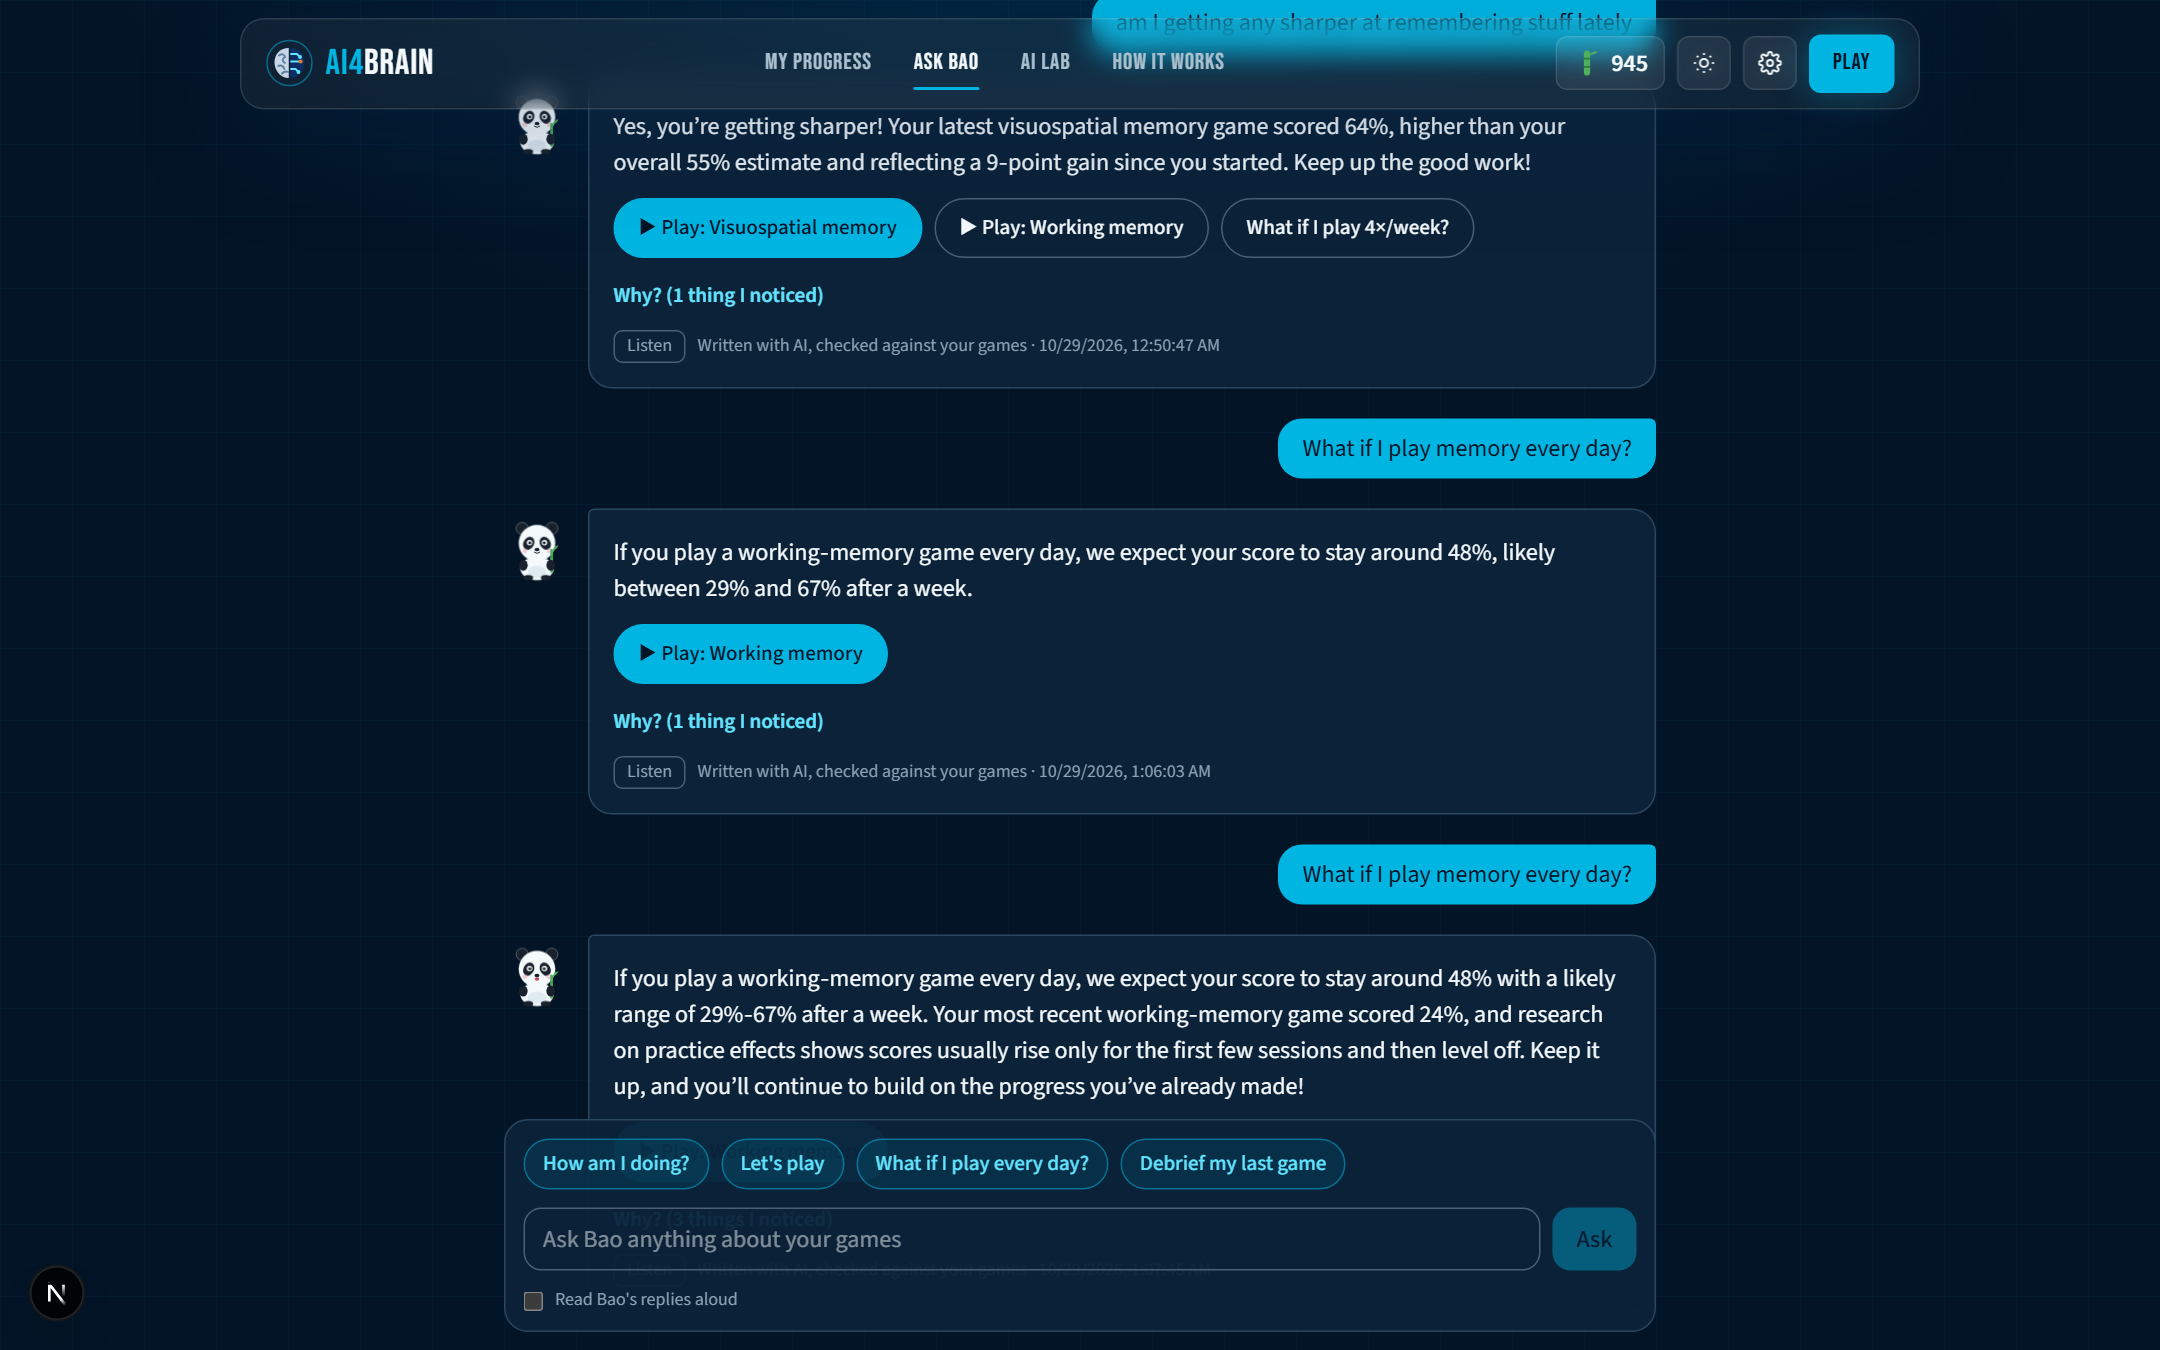
\includegraphics[height=6.6cm]{shots/coach.png}\end{center}
\vspace{0.2cm}
{\small\color{muted} Bao, the AI coach, answering ``What if I play memory every day?'' in the running application.}
\end{titlepage}

\setcounter{tocdepth}{2}
\tableofcontents
\newpage

% ---------------------------------------------------------------- 1
\section{Introduction: where AI belongs}

A cognitive coach has two very different jobs. It must \emph{measure}: turn a minute of play into a skill estimate that is accurate and honest about its uncertainty. And it must \emph{talk}: understand what a person asks, explain results in plain words and keep them motivated. Today's language models are excellent at the second job and unreliable at the first: they write fluently, but they miscount, drift between runs and cannot attach a calibrated probability to an estimate.

AI4Brain is built on that observation. \textbf{Each kind of AI does the job it is good at, and code checks the seams between them}:
\begin{itemize}
\item \aitag{gen}{Generative AI} reads and writes language: it understands the user's message, drafts the coach's answer, and argues or fabricates on purpose in two training games.
\item \aitag{prob}{Probabilistic AI} does the measuring: a Bayesian model of each skill and an active-learning selector that chooses the most informative next game.
\ifcamera\item \aitag{per}{Perception AI} runs on the device: a face-landmark model that only answers ``were the player's eyes on the screen?''.\fi
\item \aitag{guard}{Guardrails} are deterministic: schema validation, an evidence-and-number verifier, a clinical-language filter and rule-based fallbacks for every model.
\end{itemize}
Sections~\ref{sec:map}--\ref{sec:dataflow} describe each AI component, how it works and why we chose it. Section~\ref{sec:engine} summarises the measurement engine, Section~\ref{sec:validation} the evidence that it works, and Appendix~\ref{app:formulas} collects the formulas.

% ---------------------------------------------------------------- 2
\section{The AI map}
\label{sec:map}

\begin{figure}[h]
\centering
\begin{tikzpicture}[x=1cm,y=1cm]
% band labels
\node[lbl,anchor=east,text width=2.5cm,align=right,color=gen] at (1.75,0) {\textbf{Generative AI}\\LLMs, server};
\node[lbl,anchor=east,text width=2.5cm,align=right,color=prob] at (1.75,-1.75) {\textbf{Probabilistic AI}\\engine, server};
\node[lbl,anchor=east,text width=2.5cm,align=right,color=per] at (1.75,-3.5) {\textbf{Perception AI}\\on the device};
\node[lbl,anchor=east,text width=2.5cm,align=right,color=guard] at (1.75,-5.25) {\textbf{Guardrails}\\deterministic code};
% generative
\node[aibox=gen] at (3.55,0) {Intent router\\\scriptsize what to compute};
\node[aibox=gen] at (7.0,0) {Coach writer\\\scriptsize cited explanations};
\node[aibox=gen] at (10.45,0) {Persuader\\\scriptsize argues true or false};
\node[aibox=gen] at (13.9,0) {Fabricator\\\scriptsize invents one fake fact};
% probabilistic
\node[aibox=prob] at (3.55,-1.75) {Brain Twin\\\scriptsize Bayesian skill model};
\node[aibox=prob] at (7.0,-1.75) {Game selector\\\scriptsize active learning};
\node[aibox=prob] at (10.45,-1.75) {Forecaster\\\scriptsize trend with a band};
\node[aibox=prob] at (13.9,-1.75) {Simulated advisor\\\scriptsize Second opinion game};
% perception
\ifcamera
\node[aibox=per] at (3.55,-3.5) {Focus Guard\\\scriptsize face landmarks};
\node[aibox=per] at (7.0,-3.5) {Speech to text\\\scriptsize browser, optional};
\node[aibox=per] at (10.45,-3.5) {Text to speech\\\scriptsize browser, optional};
\else
\node[aibox=per] at (3.55,-3.5) {Speech to text\\\scriptsize browser, optional};
\node[aibox=per] at (7.0,-3.5) {Text to speech\\\scriptsize browser, optional};
\fi
% guardrails
\node[aibox=guard] at (3.55,-5.25) {Schema validation\\\scriptsize JSON schema, menus};
\node[aibox=guard] at (7.0,-5.25) {Evidence verifier\\\scriptsize claims and numbers};
\node[aibox=guard] at (10.45,-5.25) {Clinical filter\\\scriptsize and norm filter};
\node[aibox=guard] at (13.9,-5.25) {Rule fallbacks\\\scriptsize for every model};
\end{tikzpicture}
\caption{Every AI component in AI4Brain, grouped by kind. Language models never compute a number, a score or a diagnosis: those come from the probabilistic engine, and the guardrails enforce it.}
\label{fig:map}
\end{figure}

\begin{table}[h]
\centering\small
\caption{The AI components. ``Sees'' is everything the component receives.}
\label{tab:components}
\begin{tabularx}{\linewidth}{@{}>{\raggedright}p{2.35cm} >{\raggedright}p{3.1cm} >{\raggedright}X >{\raggedright}p{2.5cm} >{\raggedright\arraybackslash}p{2.6cm}@{}}
\toprule
Component & Model / technique & Sees $\rightarrow$ produces & Runs & Fallback\\
\midrule
Intent router & Claude or \code{gpt-oss-120b} (Groq), strict JSON & the user's message $\rightarrow$ one menu item, a skill, a pace & server, 6\,s budget & keyword rules\\
Coach writer & same providers, strict JSON & evidence pack without identifiers $\rightarrow$ reply, 0--3 cited claims, buttons & server & template coach\\
Persuader & same providers & a trivia question and a side $\rightarrow$ 70-word argument + technique & server & pre-written argument\\
Fabricator & same providers & a topic and 3 true facts $\rightarrow$ one plausible fake & server & pre-written fake\\
Brain Twin & 1-D Kalman filter & game observations $\rightarrow$ mean and 90\% band & server & n/a (exact)\\
Game selector & expected information gain & current bands $\rightarrow$ next game + reason & server & n/a\\
Forecaster & Bayesian linear trend & skill history $\rightarrow$ range at 7 days & server & n/a\\
\ifcamera Focus Guard & MediaPipe Face Landmarker (WASM) & camera frames $\rightarrow$ one boolean per trial & device only & guard off\\ \fi
Speech I/O & Web Speech API & speech $\leftrightarrow$ text & browser & typing\\
\bottomrule
\end{tabularx}
\end{table}

\subsubsection{One interface, two providers} All language-model calls go through one module with two interchangeable back ends: Claude (Anthropic) when an Anthropic key is set, otherwise the open-weight \code{gpt-oss-120b} served by Groq; a single setting forces either. Both are called with \emph{strict JSON-schema structured output}, so a reply that does not match the schema is rejected before any code reads it. Calls never throw: every failure returns a reason, and the caller switches to its rule-based fallback, so the product works with no AI provider at all.

% ---------------------------------------------------------------- 3
\section{Why these AI choices}
\label{sec:why}

Each AI decision was made against concrete alternatives. Table~\ref{tab:decisions} records them, because the rejected options are as informative as the chosen ones.

\begin{table}[h]
\centering\small
\caption{Design decisions for the AI, and the alternatives we rejected.}
\label{tab:decisions}
\begin{tabularx}{\linewidth}{@{}>{\raggedright}p{3.3cm} >{\raggedright}p{3.6cm} >{\raggedright\arraybackslash}X@{}}
\toprule
We chose & Instead of & Because\\
\midrule
LLMs for language only & an LLM that scores games or estimates skills & LLMs miscount, vary between runs and give no calibrated uncertainty; the Bayesian engine is exact, reproducible and was validated (Section~\ref{sec:validation}).\\
A bounded pipeline: at most 2 model calls & an open agent loop with tools & An agent makes 3--6 calls per question: 5--15\,s latency and free-tier rate limits during a live demo, and behaviour no deterministic test can cover. The bounded design answers in about 2\,s and is fully tested.\\
An AI router over a fixed menu & keyword rules alone & Keywords miss indirect wording (Table~\ref{tab:router}); a menu keeps the model from asking for anything the engine cannot compute.\\
Retrieval from the user's own data and 13 vetted findings & open-web retrieval or the model's memory & Every sentence must be traceable to the user's games or a reviewed paper; open retrieval cannot be verified per claim.\\
A deterministic verifier & an LLM-as-judge & A second model can hallucinate too; string-and-number checks cannot, and run in milliseconds.\\
Hosted frontier and open-weight models & fine-tuning a small local model & No GPU on the target laptop, no real conversations to learn from yet, and the verifier already catches model errors. Distillation is a later step (Section~\ref{sec:limits}).\\
Truth from a vetted bank in the AI Lab & letting the model decide what is true & The score must never depend on the model being right; testing showed a model can slip a false detail into ``true'' text.\\
Bayesian skill model & a neural network & 500 simulated users, no real data, and the need for calibrated 90\% bands: a conjugate model is the right size.\\
\ifcamera On-device perception, one bit per trial & cloud vision, or emotion recognition & Images never leave the device; and facial expressions do not reliably reveal emotions~\cite{barrett}, so we infer none.\\ \fi
\bottomrule
\end{tabularx}
\end{table}

% ---------------------------------------------------------------- 4
\section{The AI coach}
\label{sec:coach}

Bao answers questions, debriefs games, starts the right game and looks ahead. Figure~\ref{fig:sequence} shows one question end to end.

\begin{figure}[h]
\centering
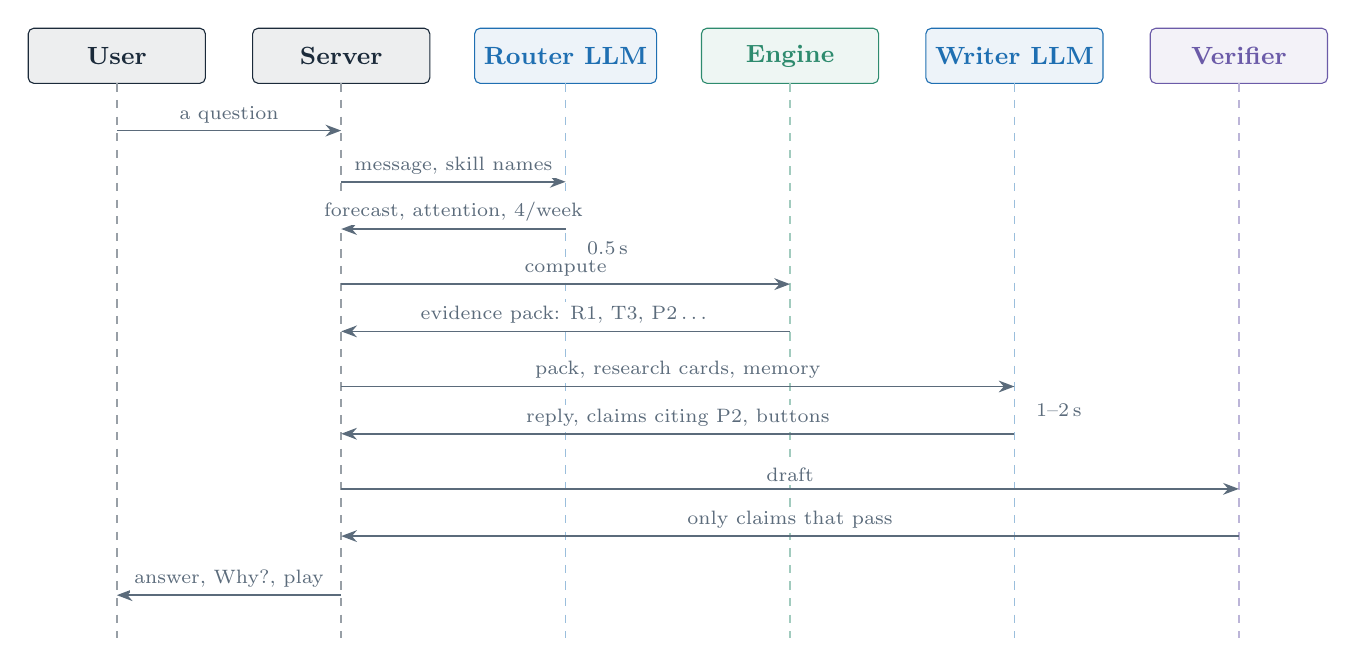
\begin{tikzpicture}[x=1cm,y=1cm,font=\small]
\foreach \x/\name/\c in {0/User/ink, 2.85/Server/ink, 5.7/Router LLM/gen, 8.55/Engine/prob, 11.4/Writer LLM/gen, 14.25/Verifier/guard} {
  \node[draw=\c,fill=\c!8,rounded corners=2pt,minimum width=2.25cm,minimum height=0.7cm,font=\small\bfseries,text=\c] at (\x,0) {\name};
  \draw[color=\c!45,line width=0.6pt,dashed] (\x,-0.35) -- (\x,-7.4);
}
\draw[flow] (0,-0.95) -- node[tagl,above=1pt]{a question} (2.85,-0.95);
\draw[flow] (2.85,-1.6) -- node[tagl,above=1pt]{message, skill names} (5.7,-1.6);
\draw[flow] (5.7,-2.2) -- node[tagl,above=1pt]{forecast, attention, 4/week} (2.85,-2.2);
\draw[flow] (2.85,-2.9) -- node[tagl,above=1pt]{compute} (8.55,-2.9);
\draw[flow] (8.55,-3.5) -- node[tagl,above=1pt]{evidence pack: R1, T3, P2\,\ldots} (2.85,-3.5);
\draw[flow] (2.85,-4.2) -- node[tagl,above=1pt]{pack, research cards, memory} (11.4,-4.2);
\draw[flow] (11.4,-4.8) -- node[tagl,above=1pt]{reply, claims citing P2, buttons} (2.85,-4.8);
\draw[flow] (2.85,-5.5) -- node[tagl,above=1pt]{draft} (14.25,-5.5);
\draw[flow] (14.25,-6.1) -- node[tagl,above=1pt]{only claims that pass} (2.85,-6.1);
\draw[flow] (2.85,-6.85) -- node[tagl,above=1pt]{answer, Why?, play} (0,-6.85);
\node[lbl,anchor=west] at (5.85,-2.45) {0.5\,s};
\node[lbl,anchor=west] at (11.55,-4.5) {1--2\,s};
\end{tikzpicture}
\caption{One coach answer. Two model calls (blue) are fenced by the engine, which computes every number (green), and the verifier, which checks everything the writer says (purple).}
\label{fig:sequence}
\end{figure}

\subsection{Step 1: the intent router}
With the user's consent, one structured call reads the message and chooses \emph{what to compute} from a fixed menu: debrief, progress, forecast (at 2, 4 or 7 games a week), goal, explain, play, help or chat, plus the skill concerned. The JSON schema allows nothing else; an off-menu intent or an invented skill id is rejected in code. Any failure, or more than 6 seconds, falls back to keyword rules with typo tolerance. Table~\ref{tab:router} shows why the AI earns its place.

\begin{table}[h]
\centering\small
\caption{Router evaluation on indirect wording, against the live model (about 0.3--0.6\,s per call).}
\label{tab:router}
\begin{tabularx}{\linewidth}{@{}X >{\raggedright}p{3.6cm} >{\raggedright\arraybackslash}p{4.6cm}@{}}
\toprule
Message & Keyword rules & AI router\\
\midrule
``am I getting any sharper at remembering stuff lately'' & chat (missed) & progress \textperiodcentered{} working memory\\
``if I did this three times a week would my focus get better'' & play (wrong) & forecast \textperiodcentered{} attention \textperiodcentered{} 4/week\\
``why do I keep messing up when the rules change mid-game'' & explain, no skill & explain \textperiodcentered{} cognitive flexibility\\
``what's the deal with that trust-the-robot game'' & play (wrong) & explain \textperiodcentered{} AI reliance\\
``I'm wiped out today, should I even bother playing?'' & chat & chat\\
``can this tell me if I have ADHD'' & chat & chat (then the clinical filter answers)\\
\bottomrule
\end{tabularx}
\end{table}

\subsection{Step 2: retrieval from the user's own data}
The engine builds an \emph{evidence pack}, the only material the writer may use: skill scores with bands, the last six games with metrics and reliability, grouped trial facts (``5 matches you caught''), exact ``what it would take'' recalculations (``1 more match caught $\rightarrow$ 68\% instead of 60\%''), forecasts at three paces, and up to 8 of 13 reviewed research findings selected for the topic. Each item has a short reference (R1, T3, W2, P1, S4). No name or database id leaves the server; the last 12 messages and a small memory (goal, favourite skill, recent topics) keep the conversation coherent without repeating itself.

\subsection{Step 3: the writer}
The writer receives the pack and a system prompt of explicit rules: cite at least one R/T/W/P reference per claim, use only numbers in the pack, mention the band with any estimate, compare the user only with their own past, never use medical terms, and keep the reply to three sentences. It returns structured JSON: an intent, a reply, 0--3 claims (each with a ``why'' and references), up to 3 action buttons and Bao's mood.

\subsection{Step 4: the verifier}
The verifier is the reason the coach can be trusted. In code, without a second model:
\begin{enumerate}
\item map every cited reference back to a game or trial group; \textbf{drop a claim with no valid evidence}, or backed only by research findings (``science explains, your data decides'');
\item extract every number from the claim and accept it only if it appears in the evidence that claim cites, within rounding ($\pm1$ for values $\ge10$, $\pm0.05$ below), or is the difference of two such numbers; dates are removed first so their digits cannot vouch for anything;
\item remove diagnostic terms and comparisons with other people; a health question receives a fixed, kind, non-clinical answer first;
\item accept only buttons that name real skills.
\end{enumerate}
This is a deterministic chain-of-verification~\cite{cove}: it cannot itself hallucinate, and the user can perform the same check by tapping ``Why?''. In an opt-in research mode, about 35\% of debriefs carry one deliberate, always-revealed number error, so that \emph{checking the AI} becomes measurable.

\subsection{When there is no AI}
Without consent, provider or network, the same intents are answered by a template coach with six or more phrasings per intent, through the same verifier. The user always gets an answer; it is simply less fluent.

% ---------------------------------------------------------------- 5
\section{AI that trains people to judge AI}
\label{sec:collab}

Relying on AI well is treated as a skill to measure and train, in three games.

\subsection{Second opinion: a simulated advisor}
The player picks the larger of two sums under time pressure, sees an AI helper's answer, then decides again. The helper is a \emph{simulated} advisor whose accuracy is controlled per trial, so that both kinds of disagreement occur in every game. Following~\cite{schemmer}, only disagreements are scored: keeping a right answer when the helper is wrong, and switching to the helper when it is right. ``Always follow'' and ``always keep'' both score at chance.

\subsection{The AI Lab: two games against a live model}
Persuasive AI is real: GPT-4 with a few personal facts won 64\% of the debates that had a clear winner~\cite{salvi}. And practising against named manipulation techniques builds resistance~\cite{roozenbeek}. The AI Lab turns both findings into games played against the live model (Figure~\ref{fig:lab}).

\begin{figure}[h]
\centering
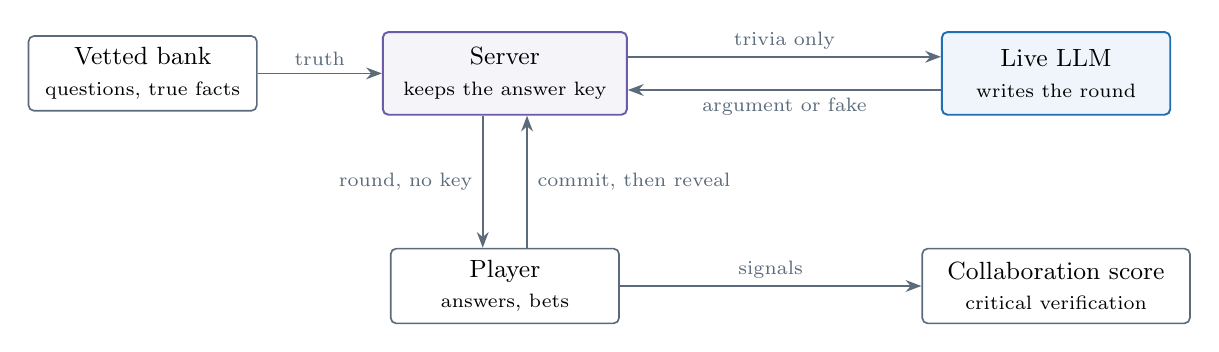
\begin{tikzpicture}[x=1cm,y=1cm]
\node[plain,minimum width=2.9cm] (bank) at (0,0) {Vetted bank\\\scriptsize questions, true facts};
\node[ai=guard,minimum width=3.1cm] (srv) at (4.6,0) {Server\\\scriptsize keeps the answer key};
\node[ai=gen,minimum width=2.9cm] (llm) at (11.6,0) {Live LLM\\\scriptsize writes the round};
\node[plain,minimum width=2.9cm] (player) at (4.6,-2.7) {Player\\\scriptsize answers, bets};
\node[plain,minimum width=3.4cm] (score) at (11.6,-2.7) {Collaboration score\\\scriptsize critical verification};
\draw[flow] (bank) -- node[tagl,above=1pt]{truth} (srv);
\draw[flow] ([yshift=6pt]srv.east) -- node[tagl,above=1pt]{trivia only} ([yshift=6pt]llm.west);
\draw[flow] ([yshift=-6pt]llm.west) -- node[tagl,below=1pt]{argument or fake} ([yshift=-6pt]srv.east);
\draw[flow] ([xshift=-8pt]srv.south) -- node[tagl,left=2pt]{round, no key} ([xshift=-8pt]player.north);
\draw[flow] ([xshift=8pt]player.north) -- node[tagl,right=2pt]{commit, then reveal} ([xshift=8pt]srv.south);
\draw[flow] (player.east) -- node[tagl,above=1pt]{signals} (score.west);
\end{tikzpicture}
\caption{AI Lab architecture. The model writes every round live, but the truth always comes from the vetted bank and the answer key stays on the server until the player commits.}
\label{fig:lab}
\end{figure}

\subsubsection{Resist the Persuader} The player answers a surprising question (``Can you see the Great Wall from space?''). The model then argues, half the time for the truth with checkable evidence, half the time for the wrong answer with one named technique: fake expert, false precision, bandwagon, vivid story or cherry-picking. The server decides which side the model argues and overrides its label: a true side is always ``real evidence''. After the final answer the reveal names the technique (prebunking). Only rounds where the model argued against the first answer count, so the score is a \emph{discernment} rate in the sense of~\cite{pennycook}.

\subsubsection{Fabrication Hunt} Three true sentences from the bank are shown word for word; the model invents one plausible, clearly false sentence on the same topic, and the server places it at a random position. The player picks the fake and wagers 1--3 tokens: post-decision wagering measures whether people know when they are right~\cite{persaud}. Testing shaped this design: when the model was allowed to reword the true facts, it once slipped in a false detail (``the shortest day of any planet''), which would have marked a correct player wrong. True sentences are therefore never rewritten, and the model is asked for fakes that are unambiguously false (a wrong date, count or name) rather than approximately true.

\begin{figure}[h]
\centering
\begin{subfigure}{0.49\linewidth}\centering\shot{\linewidth}{persuader}\caption{Resist the Persuader}\end{subfigure}\hfill
\begin{subfigure}{0.49\linewidth}\centering\shot{\linewidth}{hunt}\caption{Fabrication Hunt}\end{subfigure}
\caption{The AI Lab in the running application. Live AI writes both rounds in about half a second.}
\end{figure}

\subsection{The AI Collaboration Score}
How well the user works with AI is scored from 19 concrete signals: opening the evidence behind a claim, follow-up questions, predicting a result before asking the AI, staying within the coach's scope, catching a deliberate error, and the three games above. Each signal belongs to one of five components weighted as in the brief (clarification 20\%, critical verification 25\%, iteration 20\%, autonomy 20\%, responsible use 15\%), with Bayesian smoothing so a few interactions cannot swing the score (Appendix~\ref{app:formulas}). The AI Lab feeds this score rather than the calibrated skill estimates: live text varies between rounds, which would invalidate a measurement model.

\ifcamera
% ---------------------------------------------------------------- perception
\section{Perception AI: Focus Guard}
\label{sec:focus}

A notification glanced at mid-game silently drags a score down. Focus Guard asks the camera exactly one question per trial: \emph{were the player's eyes on the screen?}

\begin{figure}[h]
\centering
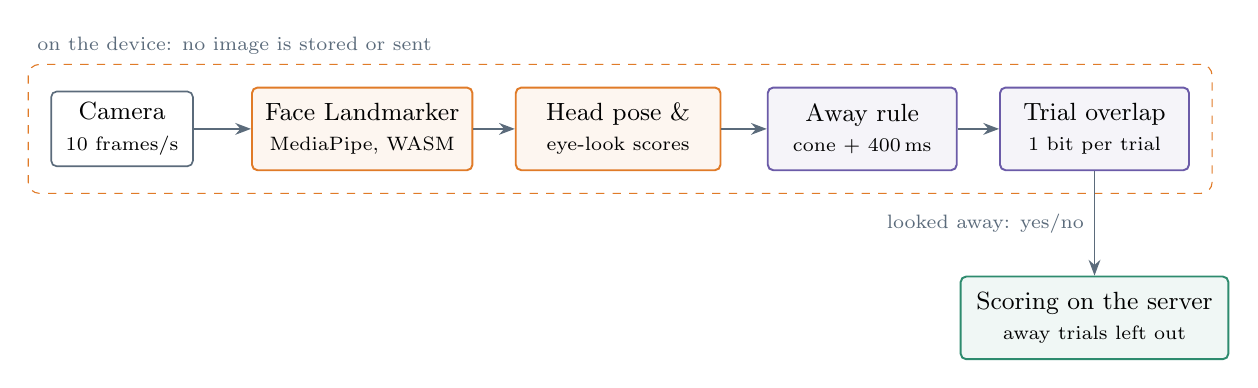
\begin{tikzpicture}[x=1cm,y=1cm]
\node[plain,minimum width=1.8cm] (cam) at (0,0) {Camera\\\scriptsize 10 frames/s};
\node[ai=per,minimum width=2.8cm] (mp) at (3.05,0) {Face Landmarker\\\scriptsize MediaPipe, WASM};
\node[ai=per,minimum width=2.6cm] (pose) at (6.3,0) {Head pose \&\\\scriptsize eye-look scores};
\node[ai=guard,minimum width=2.4cm] (rule) at (9.4,0) {Away rule\\\scriptsize cone + 400\,ms};
\node[ai=guard,minimum width=2.4cm] (trial) at (12.35,0) {Trial overlap\\\scriptsize 1 bit per trial};
\node[ai=prob,minimum width=3.4cm] (srv) at (12.35,-2.4) {Scoring on the server\\\scriptsize away trials left out};
\begin{scope}[on background layer]
\node[draw=per,dashed,rounded corners=4pt,fit=(cam)(trial),inner sep=8pt,label={[lbl,anchor=south west]north west:on the device: no image is stored or sent}] {};
\end{scope}
\draw[flow] (cam) -- (mp);
\draw[flow] (mp) -- (pose);
\draw[flow] (pose) -- (rule);
\draw[flow] (rule) -- (trial);
\draw[flow] (trial) -- node[tagl,left=2pt]{looked away: yes/no} (srv);
\end{tikzpicture}
\caption{Focus Guard. Everything inside the dashed box runs in the browser; only one boolean per trial reaches the server, and only with the camera consent.}
\label{fig:focus}
\end{figure}

\subsubsection{How it works} Google's MediaPipe Face Landmarker~\cite{mediapipe} runs in the browser as WebAssembly; the model and runtime are served by the application itself, so the strict content-security policy holds and no third party is contacted. Ten times a second, head yaw and pitch are read from the model's facial transformation matrix and eye direction from its eye-look blendshapes. A frame is \emph{looking away} when no face is found, $|\text{yaw}|>28^\circ$, $|\text{pitch}|>22^\circ$, or an eye-look score exceeds 0.65 (looking down to the keyboard counts at half weight). Spells under 400\,ms are ignored, so blinks and quick glances do not count. A trial is \emph{away} when its live window, from stimulus to response, overlaps a spell.

\subsubsection{Why this design} The camera is the most sensitive sensor a learning app can use, so its job is reduced to the minimum that improves data quality. Away trials are excluded like too-fast answers, and a game is flagged when more than 25\% of its trials were away. Because it only removes bad trials, the calibrated measurement model is unchanged. It is off by default with its own consent, the app works identically without it, and it never infers emotion, fatigue or identity.

\subsubsection{Status} Built, unit-tested, and tested end to end in a browser with a simulated camera; the thresholds are still to be tuned on real faces and lighting.
\fi

\ifcamera\subsection*{Voice}\else\section{Perception AI: voice}\fi
Questions can be dictated and answers read aloud with the browser's built-in Web Speech API. Dictation needs its own consent; the user reviews the transcript before sending, and no audio is stored. Voice is only an input method: nothing is inferred from it.

% ---------------------------------------------------------------- data flow
\section{What each AI sees}
\label{sec:dataflow}

Privacy for AI is a question of data flow. Table~\ref{tab:dataflow} lists, for every model, exactly what reaches it.

\begin{table}[h]
\centering\small
\caption{Data flow to each AI component.}
\label{tab:dataflow}
\begin{tabularx}{\linewidth}{@{}>{\raggedright}p{2.6cm} >{\raggedright}X >{\raggedright}p{2.6cm} >{\raggedright\arraybackslash}p{2.6cm}@{}}
\toprule
AI & Receives & Never receives & Requires\\
\midrule
Intent router & the question text and the list of skill names & name, id, scores & AI-coaching consent\\
Coach writer & evidence pack with short references, research cards, recent conversation & name, database ids & AI-coaching consent\\
Persuader, Fabricator & trivia from the vetted bank & anything about the player & nothing personal is sent\\
\ifcamera Focus Guard & camera frames, on the device only & (server) any image or landmark & camera consent\\ \fi
Speech to text & the user's speech, in the browser (the browser may use its own service) & & microphone consent\\
\bottomrule
\end{tabularx}
\end{table}

Personal fields stored by the app (name, coach memory and conversation, behaviour signals) are encrypted per user with AES-256-GCM under a key that belongs to that profile alone, wrapped by a master key outside the database; deleting a profile destroys its key, so even backups become unreadable. Sign-in uses passkeys or a random backup key, never an email or password. Details and the threat model are in Appendix~\ref{app:formulas} and the security documentation.

% ---------------------------------------------------------------- engine
\section{The measurement engine (probabilistic AI)}
\label{sec:engine}

\subsection{From trials to an observation}
Seven skills are measured with classic paradigms that run in about a minute each (Table~\ref{tab:tasks}). A game's metrics are normalised and weighted into a composite $c\in[0,1]$, which a calibrated level range turns into one observation on a common ability scale, so harder levels count for more. Games with too few valid trials, chance-level accuracy, long identical-answer streaks, many anticipations or timeouts, or repeated focus loss\ifcamera{} or looking away\fi{} are flagged and count with 2.5$\times$ the noise.

\begin{table}[h]
\centering\small
\caption{Skills, tasks and primary measures.}
\label{tab:tasks}
\begin{tabularx}{\linewidth}{@{}l l X l@{}}
\toprule
Skill & Task & Primary measures & Reference\\
\midrule
Working memory & Letter $N$-back (1/2/3) & $d'$ (log-linear corrected), hit RT & \cite{kirchner,owen}\\
Attention \& inhibition & Colour-word Stroop & proportional interference & \cite{stroop,macleod}\\
Processing speed & Symbol-digit coding & correct per minute, accuracy & \cite{smith,salthouse}\\
Cognitive flexibility & Parity/magnitude switching & proportional switch cost & \cite{rogers}\\
Visuospatial memory & Corsi blocks & span, total score & \cite{corsi,kessels}\\
Reasoning & Generated 3$\times$3 matrices & accuracy & \cite{raven,matzen}\\
AI reliance & Second opinion & appropriate reliance & \cite{schemmer}\\
\bottomrule
\end{tabularx}
\end{table}

\subsection{The Brain Twin}
Each skill is a Normal belief updated by a precision-weighted (one-dimensional Kalman) rule; between sessions the band widens with a drift of 0.02 per day, because ability can change. The user sees the estimate and its 90\% band in words: ``fairly sure it is between 55 and 68''.

\begin{figure}[h]
\centering\fig{\linewidth}{twin_update}
\caption{One skill's estimate for a simulated user: the band narrows with each game and widens during a six-day gap.}
\end{figure}

\subsection{Active learning and forecasts}
For every skill, task and level, the selector computes how much one more game would narrow the band and plays the largest gain, with a plain reason (``We're least sure about your attention so far ($\pm$33\%). One Stroop game at level 2 should bring that to about $\pm$18\%.''). Training instead targets the weakest skill at the level with about 75\% expected success. A Bayesian linear trend gives a 7-day forecast \emph{range}, and the dashboard later checks each forecast against the real estimate.

% ---------------------------------------------------------------- validation
\section{Validation}
\label{sec:validation}

500 simulated users with known abilities played 18 games each through the \emph{real} selector, scoring and profiler; calibration was fitted on 250 and every result is reported on the other 250. The first run's bands covered the truth only 52--82\% of the time; fitting a measurement model per level fixed it (Figure~\ref{fig:coverage}).

\begin{figure}[h]
\centering\fig{\linewidth}{coverage}
\caption{90\% band coverage on held-out users, before and after calibration. Every skill lands at 89--95\%.}
\label{fig:coverage}
\end{figure}

\begin{figure}[h]
\centering
\begin{subfigure}{0.49\linewidth}\centering\fig{\linewidth}{adaptive}\caption{Active learning vs random order}\end{subfigure}\hfill
\begin{subfigure}{0.49\linewidth}\centering\fig{\linewidth}{reliance}\caption{Second opinion: blind vs calibrated}\end{subfigure}
\caption{Left: adaptive game choice is 10\% more accurate than random order at equal effort. Right: blind strategies toward the AI advisor score at chance; calibrated players score well.}
\end{figure}

\begin{figure}[h]
\centering
\begin{subfigure}{0.49\linewidth}\centering\fig{\linewidth}{robustness}\caption{Invalid play detection}\end{subfigure}\hfill
\begin{subfigure}{0.49\linewidth}\centering\fig{\linewidth}{fairness}\caption{Bias by circumstance}\end{subfigure}
\caption{Left: 98\% of random, same-key, no-response and too-fast play is flagged, with 0--2\% false alarms. Right: proportional costs keep a slower but equally accurate person within 2 points except on processing speed, which by design \emph{is} speed.}
\end{figure}

Seven-day forecasts (1{,}200, scored as in the TADPOLE challenge~\cite{tadpole}) have 50\% and 90\% bands holding the truth 56\% and 94\% of the time; the point forecast is no better than ``no change'' at one week, so the app presents a range, not a promise. The AI components are evaluated where they act: the router on indirect wording (Table~\ref{tab:router}), the verifier and clinical filter by 544 automated tests including a red-team set of 49 risky and 36 safe phrasings, and the AI Lab by construction (truth never comes from the model).

% ---------------------------------------------------------------- ethics
\section{Ethics and safety}

\begin{itemize}
\item \textbf{Non-clinical.} The clinical filter, a fixed answer to health questions, no population norms, and claims limited to practice on these tasks.
\item \textbf{Consent for every AI.} The coach's models, the camera and the microphone each have their own opt-in consent; the app is fully usable with all of them off.
\item \textbf{Honest AI.} The coach labels its answers (``Written with AI, checked against your games''), the AI Lab tells players the model is sometimes wrong on purpose, and research-mode errors are always revealed.
\item \textbf{No dark patterns.} Rewards for showing up, never for high scores; no loss framing or notifications; Bao stays quiet during scored games.
\end{itemize}

% ---------------------------------------------------------------- limits
\section{Limitations and next steps}
\label{sec:limits}

\begin{itemize}
\item \textbf{Simulated, not human, validation} of the engine; next, a pilot of about 30 people over two sessions to refit calibration and measure test--retest reliability.
\item \textbf{AI after data.} With real (consented) conversations, a small open model can be distilled from verified coach outputs and served locally; with real players, a learning game selector and skills that inform each other can outperform today's rules.
\item \textbf{Live-AI content.} The AI Lab's truth is fixed by construction, but an invented ``fake'' could occasionally be accidentally true; reported rounds will go to a review queue.
\item \textbf{The router} is evaluated on a small set; a larger labelled set of real questions is needed.
\ifcamera\item \textbf{Focus Guard} thresholds need tuning on real faces and lighting, laptops first, then phones.\fi
\end{itemize}

% ---------------------------------------------------------------- appendix
\appendix
\section{Formulas}
\label{app:formulas}

\subsubsection{Game score} $c=\sum_k w_k\tilde m_k$ with $\tilde m_k=\operatorname{clip}((m_k-a_k)/(b_k-a_k),0,1)$; observation $x=\text{lo}_\ell+(\text{hi}_\ell-\text{lo}_\ell)\,c$. $N$-back sensitivity $d'=\Phi^{-1}(H)-\Phi^{-1}(F)$ with $H=(\text{hits}+0.5)/(\text{targets}+1)$~\cite{hautus}. Stroop and switching costs are proportional: $(\overline{RT}_{\text{hard}}-\overline{RT}_{\text{easy}})/\overline{RT}_{\text{easy}}$.

\subsubsection{Brain Twin} Observation noise $\sigma_x=\sigma_{\text{obs}}\sqrt{n_{\text{ref}}/n_{\text{valid}}}$ ($\times2.5$ if flagged). Update
\begin{equation}
\mu'=\frac{\mu/\sigma^2+x/\sigma_x^2}{1/\sigma^2+1/\sigma_x^2},\qquad \sigma'^2=\left(\sigma^{-2}+\sigma_x^{-2}\right)^{-1},\qquad \sigma^2(t+\Delta t)=\sigma^2(t)+q^2\Delta t .
\end{equation}
Band $\mu\pm1.645\sigma$; goal probability $P(\theta\ge g)=1-\Phi((g-\mu)/\sigma)$. Calibration fits $c=a+b\theta+\varepsilon$ per level and sets $\text{lo}_\ell=-a/b$, $\text{hi}_\ell=(1-a)/b$.

\subsubsection{Active learning} The expected narrowing from one more game is $\Delta\sigma=\sigma-(\sigma^{-2}+\tilde\sigma_x^{-2})^{-1/2}$, and the weekly plan ranks skills by $0.6\,(\text{band}/\text{prior band})+0.4\,(1-\mu)$.

\subsubsection{Working with AI} Collaboration score $\operatorname{round}(100\sum_c w_c s_c)$, $s_c=(\sum v_i+0.5\cdot2)/(n_c+2)$. Appropriate reliance $\tfrac12(\text{RSR}+\text{RAIR})$. Discernment $D=\#\{\text{final correct}\wedge\text{AI disagreed}\}/\#\{\text{AI disagreed}\}$. Wager gap $G=\mathbb E[w\mid\text{caught}]-\mathbb E[w\mid\text{missed}]$.

\ifcamera\subsubsection{Focus Guard} Yaw $=\operatorname{atan2}(-r_{20},\sqrt{r_{00}^2+r_{10}^2})$, pitch $=\operatorname{atan2}(r_{21},r_{22})$ from the rotation part of the transformation matrix; $n_{\text{valid}}$ excludes away trials; flag if $\#\text{away}/n>0.25$.\fi

\subsubsection{Security} Each personal field is stored as $C=\operatorname{AES\text{-}GCM}_{K_u}(m;\ \text{aad}=\text{field})$ under the user's key, itself wrapped as $W_u=\operatorname{AES\text{-}GCM}_{M_v}(K_u)$. The security log chains $h_i=\operatorname{HMAC}_k(h_{i-1}\,\|\,e_i)$. Failed sign-ins wait $d_n=\min(250\,\text{ms}\cdot2^{\,n-3},\,8\,\text{s})$, and the chance of guessing any of $N$ backup keys in $G$ tries is $NG/2^{80}$.

% ---------------------------------------------------------------- references
\begin{thebibliography}{99}\small
\setlength{\itemsep}{0.1em}
\bibitem{barrett} L.~F.~Barrett, R.~Adolphs, S.~Marsella, A.~M.~Martinez, S.~D.~Pollak. Emotional expressions reconsidered: challenges to inferring emotion from human facial movements. \emph{Psychological Science in the Public Interest}, 20(1):1--68, 2019.
\bibitem{corsi} P.~M.~Corsi. \emph{Human memory and the medial temporal region of the brain}. PhD thesis, McGill University, 1972.
\bibitem{cove} S.~Dhuliawala et al. Chain-of-verification reduces hallucination in large language models. \emph{Findings of ACL}, 2024.
\bibitem{hautus} M.~J.~Hautus. Corrections for extreme proportions and their biasing effects on estimated values of $d'$. \emph{Behavior Research Methods, Instruments, \& Computers}, 27(1):46--51, 1995.
\bibitem{kessels} R.~P.~C.~Kessels et al. The Corsi block-tapping task: standardization and normative data. \emph{Applied Neuropsychology}, 7(4):252--258, 2000.
\bibitem{kirchner} W.~K.~Kirchner. Age differences in short-term retention of rapidly changing information. \emph{Journal of Experimental Psychology}, 55(4):352--358, 1958.
\bibitem{macleod} C.~M.~MacLeod. Half a century of research on the Stroop effect. \emph{Psychological Bulletin}, 109(2):163--203, 1991.
\bibitem{tadpole} R.~V.~Marinescu et al. TADPOLE Challenge: prediction of longitudinal evolution in Alzheimer's disease. arXiv:1805.03909, 2018.
\bibitem{matzen} L.~E.~Matzen et al. Recreating Raven's: software for systematically generating large numbers of Raven-like matrix problems. \emph{Behavior Research Methods}, 42(2):525--541, 2010.
\ifcamera
\bibitem{mediapipe} Y.~Kartynnik, A.~Ablavatski, I.~Grishchenko, M.~Grundmann. Real-time facial surface geometry from monocular video on mobile GPUs. arXiv:1907.06724, 2019.
\fi
\bibitem{owen} A.~M.~Owen, K.~M.~McMillan, A.~R.~Laird, E.~Bullmore. N-back working memory paradigm: a meta-analysis of normative functional neuroimaging studies. \emph{Human Brain Mapping}, 25(1):46--59, 2005.
\bibitem{pennycook} G.~Pennycook, D.~G.~Rand. Lazy, not biased: susceptibility to partisan fake news is better explained by lack of reasoning than by motivated reasoning. \emph{Cognition}, 188:39--50, 2019.
\bibitem{persaud} N.~Persaud, P.~McLeod, A.~Cowey. Post-decision wagering objectively measures awareness. \emph{Nature Neuroscience}, 10(2):257--261, 2007.
\bibitem{raven} J.~Raven. The Raven's progressive matrices: change and stability over culture and time. \emph{Cognitive Psychology}, 41(1):1--48, 2000.
\bibitem{rogers} R.~D.~Rogers, S.~Monsell. Costs of a predictable switch between simple cognitive tasks. \emph{Journal of Experimental Psychology: General}, 124(2):207--231, 1995.
\bibitem{roozenbeek} J.~Roozenbeek, S.~van der Linden. Fake news game confers psychological resistance against online misinformation. \emph{Palgrave Communications}, 5:65, 2019.
\bibitem{salthouse} T.~A.~Salthouse. The processing-speed theory of adult age differences in cognition. \emph{Psychological Review}, 103(3):403--428, 1996.
\bibitem{salvi} F.~Salvi, M.~Horta Ribeiro, R.~Gallotti, R.~West. On the conversational persuasiveness of GPT-4. \emph{Nature Human Behaviour}, 9(8), 2025.
\bibitem{schemmer} M.~Schemmer et al. Appropriate reliance on AI advice: conceptualization and the effect of explanations. \emph{Proc.\ IUI}, 410--422, 2023.
\bibitem{smith} A.~Smith. \emph{Symbol Digit Modalities Test: manual}. Western Psychological Services, 1982.
\bibitem{stroop} J.~R.~Stroop. Studies of interference in serial verbal reactions. \emph{Journal of Experimental Psychology}, 18(6):643--662, 1935.
\end{thebibliography}

\end{document}
